%%% -*-LaTeX-*-

\chapter{Introduction}

\setupuuchapterbib

Arithmetics in computers is finite and thus imprecise.
%
The precision format (often called \emph{bit width} in the literature) is the length of the word used to represent real numbers in machines.
%
As a general rule of thumb, the wider the precision format the more accurate are the computations.
%
Finite-precision arithmetics, like floating-point~\cite{ieee754}, with single or double precision formats, does not respect the rules of ideal arithmetic done with 'pen and paper'. 
%
The gap between the ideal and the finite-precision computation is called roundoff error, and can have catastrophic consequences on the correct execution of a program.
%
It is then critical, not only to be aware of the existence of this gap, but also to bound the difference between the two programs.
%Numerical analysis is the branch of rigorous mathematics concerning the analysis of numerical algorithms used to implement the solutions to mathematical problems~\cite{higham2002accuracy}. 
%
\section{Roundoff Error Analysis}
%
The gap between an ideal computation and the floating-point counterpart is called roundoff error, because the result of every ideal computation gets rounded to fit the finite precision format.
%
The goal of roundoff error analysis is to measure the approximation errors stemming from the floating-point implementation of a program.
%
While, in general, roundoff errors are very small, they propagate through computations and they rapidly accumulate.
%

For example, consider the program reported in Figure~\ref{fig:while}.

%
\begin{figure}[h!]
	\begin{lstlisting}[frame=single, language=Python]
n=0
t=0
while True:
	t = t + 1
	n = n + 0.1
	\end{lstlisting}
	\caption{A simple while loop showing the effect of roundoff errors.}\label{fig:while}
\end{figure}
%
After 10 seconds, the value of the variable t is 231047636, while the value of the variable n is roughly 23104763.55.
%
Ideally, the value of n should be 23104763.6.
%
There is an absolute roundoff error of 0.45 in this program.
%
Thanks to this small example, we can see how rapidly roundoff errors accumulate in loops. 
%
From an implementation perspective, a similar issue was the cause of the Patriot Missile Failure~\cite{patriot}.
%

%The goal of roundoff error analysis is to measure the approximation errors stemming from the floating-point implementation of a program.
%
%In this thesis, we focus on a so called rigorous (i.e. sound) roundoff error analysis. 
%

The approach we used to quantify the roundoff error in our example, assumes we have a reference implementation to compare with, in the literature often called the \emph{oracle}~\cite{blame}, holding the ideal value of the computation.
%
In our example, the oracle is the integer variable t.
% 
%In our small example, regardless of its simplicity, shows a critical (and limiting) assumption we are making here, to 

In real-world applications, the oracle typically consists of a clone of the original program, where all the floating-point variables (e.g., single or double) have been replace by custom multiple-precision floating-point variables~\cite{mpfr}.
%
In the latter, the user can specify the bit width of the format (e.g., 1000bits) and use this high-precision program as a proxy for the ideal (infinite precision) implementation.
%
At this point, we have two copies of the same program, one is the implementation, and the other one is the oracle. 
%
The idea is to execute both the implementation and the oracle with the same input values, and ultimately measure the arithmetic difference between the two outputs. 
%
This is going to be the forward roundoff error of the program. 
%

While the oracle based approach has been used in several successful tools~\cite{landau2014guide, kahan1996improbability, atomic, blame, herbie} it suffers from two main limitations.
%
First, implementing a high quality high-precision oracle requires much expertise, and thus is expensive in terms of development cost~\cite{atomic}.
%
Second, using Monte Carlo sampling to exhaustively search the input space results in not-rigorous (i.e. unsound) error bounds~\cite{glasserman2013monte, parker2000monte}.
%
In this thesis, we focus on rigorous (i.e. sound) roundoff error analysis.
%
We give a sound (or rigorous) guarantee if there is 100\% certainty about the guarantee.
%
%Clearly, any approach making probabilistic statements based on Monte-Carlo sampling is unsound.
%
For example, when we say 95\% of the computations obey a certain roundoff error bound $\epsilon$, we are making a sound statement based on some analytical model of the computations, and there is therefore no uncertainty about this statement.
%
A special case of rigorous error analysis is the so called \emph{worst-case} error analysis, which implies the roundoff error bound holds for any input value.

\subsection{Worst-Case Error Analysis}
\label{sec:worst}
%
In the last decade, many successful techniques have been used to implement worst-case error analysis~\cite{darulova2018daisy,2015_fm_sjrg,solovyev2018rigorous,rosa,fptuner,smartfloat,satire,gappa,fluctuat}.
%
Here, the keyword \emph{worst-case} stands for the property of the error bound to hold for \emph{any} input value.
%
This (strong) property of the error bound is precious for all those applications, like safety-critical ones~\cite{guardstable, cpralg}, where the application context makes mandatory the use of worst-case errors.
%
Intuitively, no one would feel comfortable traveling with autonomous running aircrafts which are safe 50\% of the time.

%
From an user perspective, the main advantage of worst-case error analysis is we only need to know the range of the inputs, and ignore how the inputs are distributed in such ranges. 
%
Indeed, the resulting error bounds hold for any input value, regardless of the distribution.
%
%This is why the state-of-the-art refers to this non-deterministic model as \emph{worst-case}, because it does not account for the distribution of the inputs.
%
This property is priceless, in particular, when the input distributions are unknown.
%

On the other hand, in Section \ref{sec:prob} we discuss how \emph{ignoring} the distribution of the inputs becomes a limitation when \emph{we do know} how the inputs are distributed.
%

Finally, a strict requirement of worst-case analysis is the input variables must be bounded  in a finite range. This is because, in the worst-case, unbounded variables lead to unbounded roundoff errors, which in practice, are of little use from an implementation prospective.
\subsection{Control-flow Analysis and Roundoff Errors}
%
While roundoff error analysis has been successfully used to bound straight-line expressions, less attention has been given to other common programming constructs, like conditionals~\cite{precisa, fluctuat}.
%

In error analysis, it is critical to deal with conditionals because the control-flow of a computer program evaluated in floating-point arithmetic might differ from the ideal flow in real arithmetic.
%
%For example, the condition of an if-statements evaluates to true in real arithmetic, but because of finite-precision arithmetic, the same condition evaluates to false.
%
This is a so called \emph{instability jump}~\cite{satire} or \emph{control-flow instability}~\cite{unstable}.
%
The absolute error stemming from instabilities can be measured as the arithmetic difference between the expressions in the \emph{then} and the \emph{else} branches.
%
In general, while the roundoff error of straight line expressions is in the order of \emph{machine epsilon}, an instability jump can be in the order of the units, which typically is many orders of magnitude wider than the former.
%

Consider the if-statement reported in Figure~\ref{fig:ifstatement}. 
%
\begin{figure}[h!]
	\begin{lstlisting}[frame=single, language=Python]
	if c(x)>5:
		return f(x)
	else:
		return g(x)	
	\end{lstlisting}
	\caption{A simple if-statement we use to study instabilities. c(x), f(x) and g(x) are generic expressions.}\label{fig:ifstatement}
\end{figure}
%

We set \lstinline{c(x)=x}, \lstinline{f(x)=1} and \lstinline{g(x)=-1}.
%
Moreover, we assume the variable \lstinline{x} is bounded by the closed interval $[0,10]$.

\begin{figure}[h!]
	\centering
	\begin{tabular}{ll}
		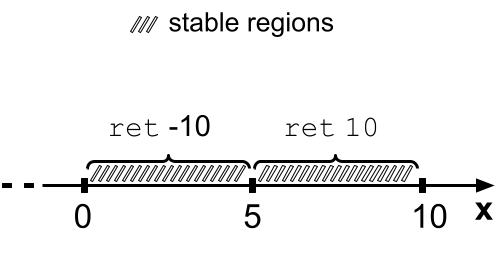
\includegraphics[width=0.5\textwidth]{pic/ifreal.png}
		&
		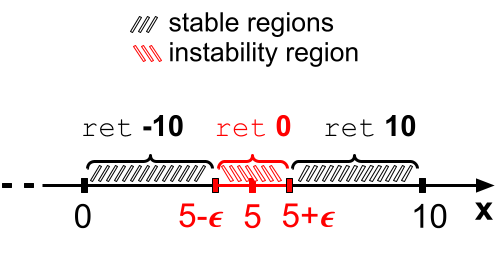
\includegraphics[width=0.5\textwidth]{pic/iffp.png}
	\end{tabular}
	\caption{A simple if-statement in case of real arithmetic (left) and the floating-point counterpart (right). In red you can see the instability region, where $\epsilon$ is the roundoff error accumulated in the variable X.}
	\label{fig:ifreal}
\end{figure}

In Figure \ref{fig:ifreal}, we plot the instability region for our small benchmark. Clearly, when we compute in real arithmetic we do not have instabilities. On the other hand, in the floating-point computations, we can identify the \emph{instability region} as that part of the input domain from where instabilities might be triggered.
%
The width of the instability region is determined by the roundoff error $\epsilon$.
%
In our small example, $\epsilon$ is the roundoff error for the variable $x$ which is proportional to $x*(2^{-p})$ where p is the bit-width of the floating-point format, and assumes maximal magnitude when $x=10$.  
%
In double precision arithmetic (64-bits), $\epsilon$ equals $1.1e^{-17}$.
%

On the other hand, the instability jump can be statically measured as $|10-(-10)|=20$. As you can see, there are about 18 orders of magnitude between the roundoff error and the instability jump error.
%
This shows how critical it is to precisely reason about roundoff errors in conditionals.
 
\subsection{Probabilistic Error Analysis}
\label{sec:prob}
%
In this section, we describe how we tackle the conservativeness of worst-case analysis, by introducing our framework to compute probabilistic (or conditional) error bounds.
%
As we mentioned in the introduction, worst-case analysis could provide conservative error bounds in case we know \emph{a priori} the distribution of the inputs. 
%
%Furthermore, we must bound the input variables to prevent overflow and thus unbounded roundoff errors.
%

In our probabilistic framework, we use probabilistic range analysis to compute conditional roundoff errors where, as opposed to the worst-case approach, the roundoff error is computed with respect to the computation landing in a given confidence interval of interest (e.g., 85\%,99\%, 99.9999\%).
%
Note, in the worst-case approach, there is an implicit 100\% confidence interval, thus worst-case analysis and 100\% confidence interval are synonyms.
%

%
Consider the program reported in Figure~\ref{fig:prob}.
%
\begin{figure}[h!]
	\begin{lstlisting}[frame=single, language=Python]
if c(x)>constant:
	return 1/0 #ERROR
else:
	return 0 #OK
	\end{lstlisting}
	\caption{A simple if-statement we use to study the conservativeness of worst-case analysis. The \emph{then} branch leads to an error while the \emph{else} branch returns correctly.}
	\label{fig:prob}
\end{figure}
%
We set \lstinline{c(x)=x}, and we assume the variable $x\sim Normal(0,1)$ is distributed accordingly to a standard normal with parameters $\mu = 0$ and $\sigma = 1$.
%

At line 1, we compare c(x) with a constant value.
%
In case the comparison evaluates to true, the \emph{then} branch leads to an error (division by zero), otherwise, the \emph{else} branch returns correctly.
%
\emph{Regardless} of the value of the constant, \emph{any} rigorous (i.e. sound) worst-case range analysis is going to signal a potential division by-zero error at line 2.
%
In simple words, the analysis is going to terminate as soon as the error is detected.
%
This is because, in case the error at line 2 is triggered the program would crash, and thus, in this situation, it would not make sense to propagate ranges or, in particular, to talk about roundoff errors.

%
A developer using such analysis has no information about \emph{how rare} might be the condition leading to such crash. 
%

In our probabilistic framework, we know the standard normal distribution concentrates more than 99\% of probability mass in the interval $[−3, 3]$, and less than 0.5\% of mass spreads in the interval $[3, \infty]$.
%
For example, in case we set constant to 1000, a developer using our combined analysis, might not be interested in the very rare outliers triggering the error at line 2.
%
Thus, if we go back to our example, we can use our probabilistic analysis with a \emph{confidence interval} set, for example, to 99\%.
%
%Clearly, other confidence intervals of interest could be used. 
%
With this setting, not only the program terminates correctly (return 0), but our probabilistic analysis bounds the roundoff error of $c(x)=x$ by $\epsilon = 3*(2^{-p})$.
%

In general, by studying the \emph{average} execution of a computer program we can prune away very rare corner cases and provide meaningful directions for an implementation prospective.
%
\section{Dissertation Statement}
%
Our thesis statement is the following: 

%
\emph{We show how to improve the stability of computer programs by encoding the mix of real and floating-point formulas in SMT solvers.
%
Moreover, in case a developer is willing to trade the accuracy of a computer program for the sake of the efficiency, we can quantify very precisely the idea of probabilistic reliability of the low-precision program.}

\section{Contributions}
%
In Chapter \ref{sec:fprock}, we describe FPRoCK (Floating-Point Real Checker), a prototype of an SMT solver we developed to reason about the mix of floating-point and real arithmetics, which is critical to spot instability jumps in computer programs.

%
%In the last decade, there has been a massive usage of low precision implementations (e.g. in artificial intelligence with CNN) primarily to conserve resources such as energy, memory footprint and execution time~\cite{lutnet}.
%
%Clearly, the high demand of resources from floating-point arithmetic is problematic, in particular, when dealing with portable devices (e.g. smart-watches) where the usage and the duration of the battery is a primary concern.
%
%Thus, the need to sacrifice the accuracy of computations in favor of the efficiency.
%
In Chapter \ref{sec:emsoft}, we describe our framework to design low precision micro-controllers.
%
We show how we can use static analysis to guarantee the stability of the micro-controller is not affected by the low-precision format.
%
Indeed, our goal is to guarantee the usage of low-precision formats does not impact the reliability of the system.

%
%InWe can use a similar argument to describe the nature of worst-case analysis. 
%

%The current state-of-the-art for roundoff error analysis have primary focused on worst-case error bounds~\cite{darulova2018daisy,2015_fm_sjrg,solovyev2018rigorous,rosa}.
%
%With the keyword \texttt{worst-case} we mean the property of the error bound to hold for \texttt{any} input value.
%
%While this is priceless in, for example, safety-critical applications~\cite{cpr}, there are a variety of (non-safety) applications where a developer might want to trade some accuracy in favor of a lower-cost precision format.
%
In Chapter \ref{sec:cav}, we describe our probabilistic error analysis, evolving from worst-case analysis, where the developer can set a custom confidence interval of interest (e.g. 85\%, 95\%, 99\%, etc.) and ignore extremely unlikely corner cases, and ultimately obtain more optimal results.
%Worst-case errors and 100\% confidence interval are synonyms.
%

\newpage
\bibliographystyle{plain}
\bibliography{\jobname}

%When we trade the accuracy of a computation for efficiency, what can we say about property of our system like stability or soundness. In alternative, in case we cannot guarantee soundness anymore, can we measure exactly how much unsoundness our application has to be able to tolerate.
%
%This is critical when we want to bound roundoff errors for programs rather than for arithmetic expressions.
%
%We use 
%

%
%Efficiently collecting data and systematically analyzing them is essential to gaining insight into the behavior of complex programs and help developers fix the flaws of the program. Also, given the rich set of concurrency primitives in modern languages, one needs to articulate nuanced concurrency coverage metrics and demonstrate their attainment.
%
%And this is my thesis statement: exact reasoning about roundoff error is hard. We can use exact reasoning for handling conditionals (like we show with FPRock). Overapproximation works for real world problem, like EMSOFT, but it is worst-case. We show how a probabilistic analysis can tackle the limitations of worst-case analyisis in real world applications.